\section{Model ve Eğitim}
\label{CH:Model}

\subsection{BiGRU temel modeli}

Temel sınıflandırıcı olarak iki katmanlı ve iki yönlü bir GRU (BiGRU) kurulmuştur~\cite{Cho2014}.
Girdi önce 100 boyuttan 256 boyuta indirgenir (doğrusal katman, ReLU, yüzde 20
dropout). Ardından iki GRU katmanı diziyi ileri ve geri yönde işler. Çıkışta son gizli
durum yerine zaman ekseni boyunca ortalama alınır ve 226 sınıfa yönelik doğrusal katman
uygulanır. Zaman ortalamasının seçilme nedeni, işaretin hangi karede bittiğinin kesin
olmaması ve dizinin başındaki ya da sonundaki boş karelerin sonucu kaydırmasının
istenmemesidir. Modelin katmanları Tablo~\ref{tab:gru} içinde verilmiştir.

\begin{table}[H]
\centering
\caption{BiGRU modelinin katmanları ve parametre sayıları}
\label{tab:gru}
\begin{tabular}{lrr}
\toprule
\textbf{Katman} & \textbf{Çıkış boyutu} & \textbf{Parametre} \\
\midrule
Girdi doğrusal katmanı & $64\times256$ & 25.856 \\
GRU katmanı 1 (iki yönlü) & $64\times512$ & 787.968 \\
GRU katmanı 2 (iki yönlü) & $64\times512$ & 1.181.184 \\
Çıkış doğrusal katmanı & 226 & 115.938 \\
\midrule
\textbf{Toplam} & & \textbf{2.114.018} \\
\bottomrule
\end{tabular}
\end{table}

\subsection{1B-CNN + Transformer modeli}

İkinci mimari, üç katmanlı 1B evrişim ağı ile iki katmanlı Transformer
kodlayıcısının~\cite{Vaswani2017} birleşimidir. Evrişim katmanları
($100\rightarrow128\rightarrow256\rightarrow256$, her birinden sonra batch
normalizasyonu ve GELU) kısa süreli yerel el hareketlerini çıkarır. İkinci evrişim
katmanındaki 2 adımlık kaydırma dizi uzunluğunu 64'ten 32'ye indirerek sonraki dikkat
hesabının maliyetini düşürür. Sinüzoidal konum kodlamasının ardından gelen Transformer
kodlayıcısı ($d_{\text{model}}=256$, 4 dikkat başlığı, ileri besleme boyutu 512, ön
normalizasyon) uzun menzilli zaman ilişkilerini öğrenir. Çıkışta yine zaman ortalaması
alınır, katman normalizasyonundan sonra 226 sınıfa doğrusal katman uygulanır. Model
1.473.634 parametreye sahiptir, yani BiGRU'dan yaklaşık yüzde 30 daha küçüktür. Ayrıca
tekrarlayan katman içermediği için eğitimi paralelleştirilebilir.

\subsection{Eğitim düzeni}

Her iki model de PyTorch ile aynı veri, aynı artırma ve aynı hiperparametrelerle
eğitilmiştir: 60 epoch, AdamW~\cite{Loshchilov2019} ($\text{lr}=2\times10^{-3}$,
ağırlık azaltımı $10^{-2}$), kosinüs öğrenme oranı azaltımı, 128'lik batch ve 0,1
etiket yumuşatma~\cite{Szegedy2016}. Doğrulama doğruluğu en yüksek olan epoch'un
ağırlıkları saklanmış, test kümesi yalnızca eğitim bittikten sonra bir kez ölçülmüştür.
Tek bir koşunun şans eseri iyi ya da kötü çıkabileceği göz önüne alınarak her model
üç farklı tohumla (0, 1, 2) eğitilmiştir. Eğitimler Apple M4 (MPS) ve NVIDIA RTX 3050
üzerinde yapılmış, tohum 0 için 60 epoch BiGRU'da 77,6 dakika, 1B-CNN + Transformer'da
18,1 dakika sürmüştür.

Kodda veri hazırlığı (\texttt{features.py}), modeller (\texttt{models.py}) ve eğitim
döngüsü (\texttt{train\_gru.py}) ayrı dosyalardadır. Her koşu
\texttt{experiments/} altına tohum, hiperparametreler, epoch bazında kayıp ve
doğrulama doğruluğu ile birlikte JSON olarak yazılmaktadır.

\subsection{Sonuçlar}

Tohum 0 ile yapılan karşılaştırma Tablo~\ref{tab:tohum0}, üç tohumun ortalaması ve
standart sapması Tablo~\ref{tab:uctohum} içinde verilmiştir. Eğitim kaybı ve doğrulama
doğruluğunun epoch'lara göre değişimi Şekil~\ref{fig:egri} üzerinde görülmektedir.

\begin{table}[H]
\centering
\caption{226 sınıfta iki modelin karşılaştırması (tohum 0, 60 epoch)}
\label{tab:tohum0}
\small
\begin{tabular}{@{}lrrrr@{}}
\toprule
\textbf{Model} & \textbf{Parametre} & \textbf{Doğrulama (\%)} & \textbf{Test (\%)} & \textbf{Macro F1 (\%)} \\
\midrule
BiGRU-2x256 & 2.114.018 & 89,23 & 88,24 & 88,09 \\
1B-CNN + Transformer & 1.473.634 & \textbf{89,97} & \textbf{88,83} & \textbf{88,61} \\
\bottomrule
\end{tabular}
\end{table}

\begin{table}[H]
\centering
\caption{Üç tohumla (0, 1, 2) test ve doğrulama doğrulukları}
\label{tab:uctohum}
\small
\setlength{\tabcolsep}{4pt}
\begin{tabular}{@{}lccc|cc@{}}
\toprule
\textbf{Model} & \textbf{Tohum 0} & \textbf{Tohum 1} & \textbf{Tohum 2} & \textbf{Test ort.\ $\pm$ ss} & \textbf{Doğr.\ ort.} \\
\midrule
BiGRU-2x256 & 88,24 & 87,81 & 87,89 & 87,98 $\pm$ 0,23 & 89,38 \\
1B-CNN + Transformer & 88,83 & 89,79 & 89,66 & \textbf{89,42 $\pm$ 0,52} & \textbf{90,37} \\
\bottomrule
\end{tabular}
\end{table}

\begin{figure}[H]
\centering
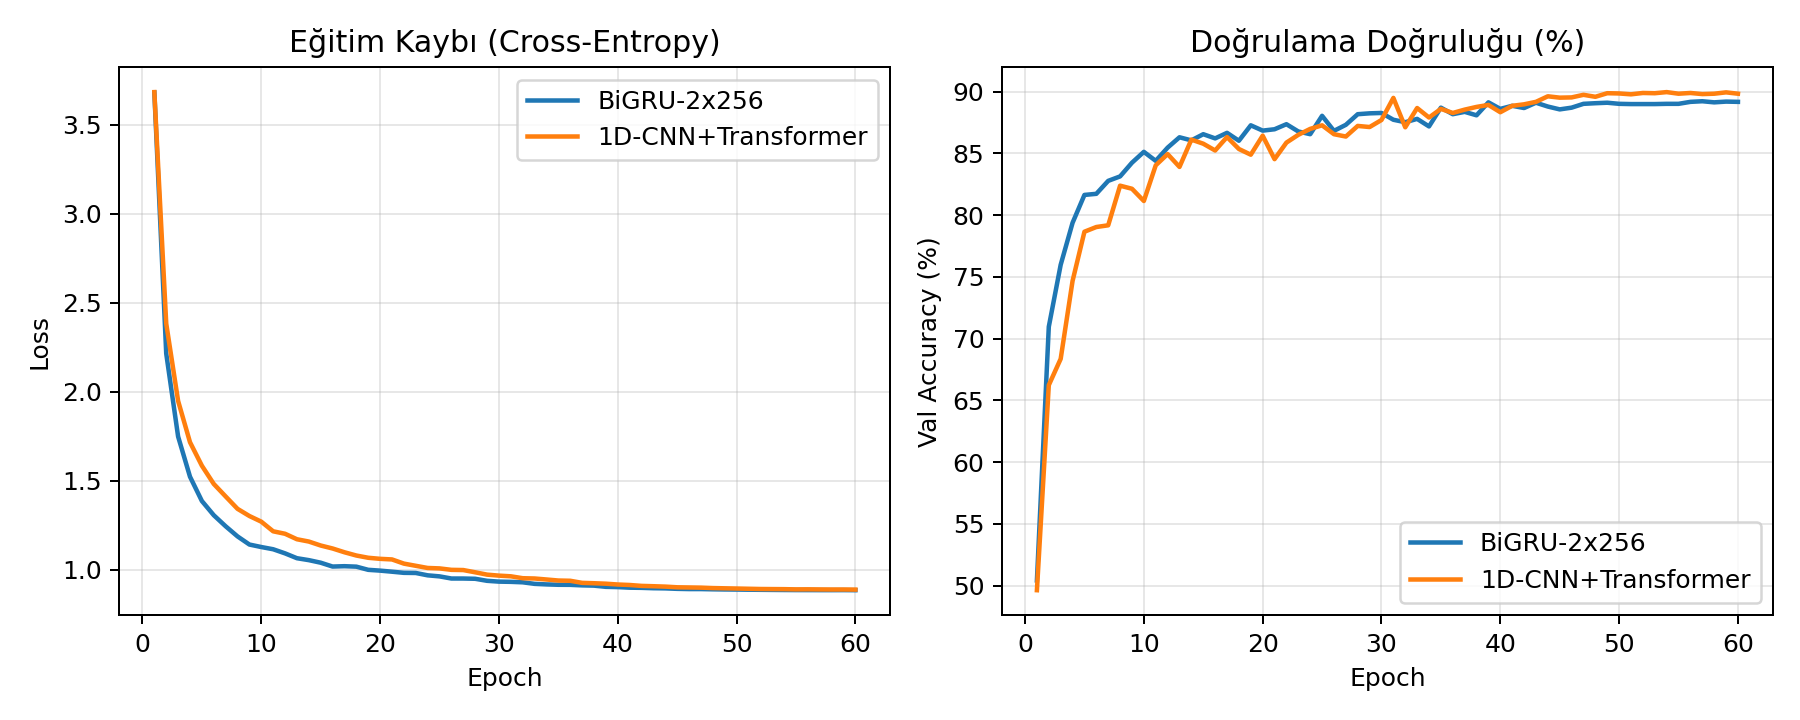
\includegraphics[width=0.95\textwidth]{grafik/egitim_egrisi.png}
\caption{İki modelin 60 epoch boyunca eğitim kaybı ve doğrulama doğruluğu (tohum 0)}
\label{fig:egri}
\end{figure}

1B-CNN + Transformer modeli üç tohumun üçünde de BiGRU'dan daha yüksek test
doğruluğuna ulaşmış, ortalamada fark yaklaşık 1,4 puan olmuştur. Şekil~\ref{fig:egri}
incelendiğinde BiGRU'nun ilk epoch'larda daha hızlı yükseldiği, ancak 30. epoch'tan
sonra Transformer tabanlı modelin öne geçtiği görülmektedir. Daha az parametreye sahip
olması, eğitiminin daha hızlı olması ve telefonda da daha küçük kalması
(Bölüm~\ref{CH:Uygulama}) nedeniyle uygulamada kullanılacak model olarak
1B-CNN + Transformer seçilmiş, üç tohum içinde doğrulama doğruluğu en yüksek olan
tohum 1 ağırlıkları alınmıştır (doğrulama yüzde 90,56, test yüzde 89,79).

\subsection{Hata analizi}

Hataların nerede toplandığını görmek için test kümesindeki 3.741 örnek üzerinde
karışıklık matrisi ve sınıf bazlı F1 skorları çıkarılmıştır
(\texttt{error\_analysis.py}). En çok karışan 18 sınıfın alt matrisi
Şekil~\ref{fig:cm}, en sık karışan işaret çiftleri Tablo~\ref{tab:karisan} içinde
verilmiştir.

\begin{figure}[H]
\centering
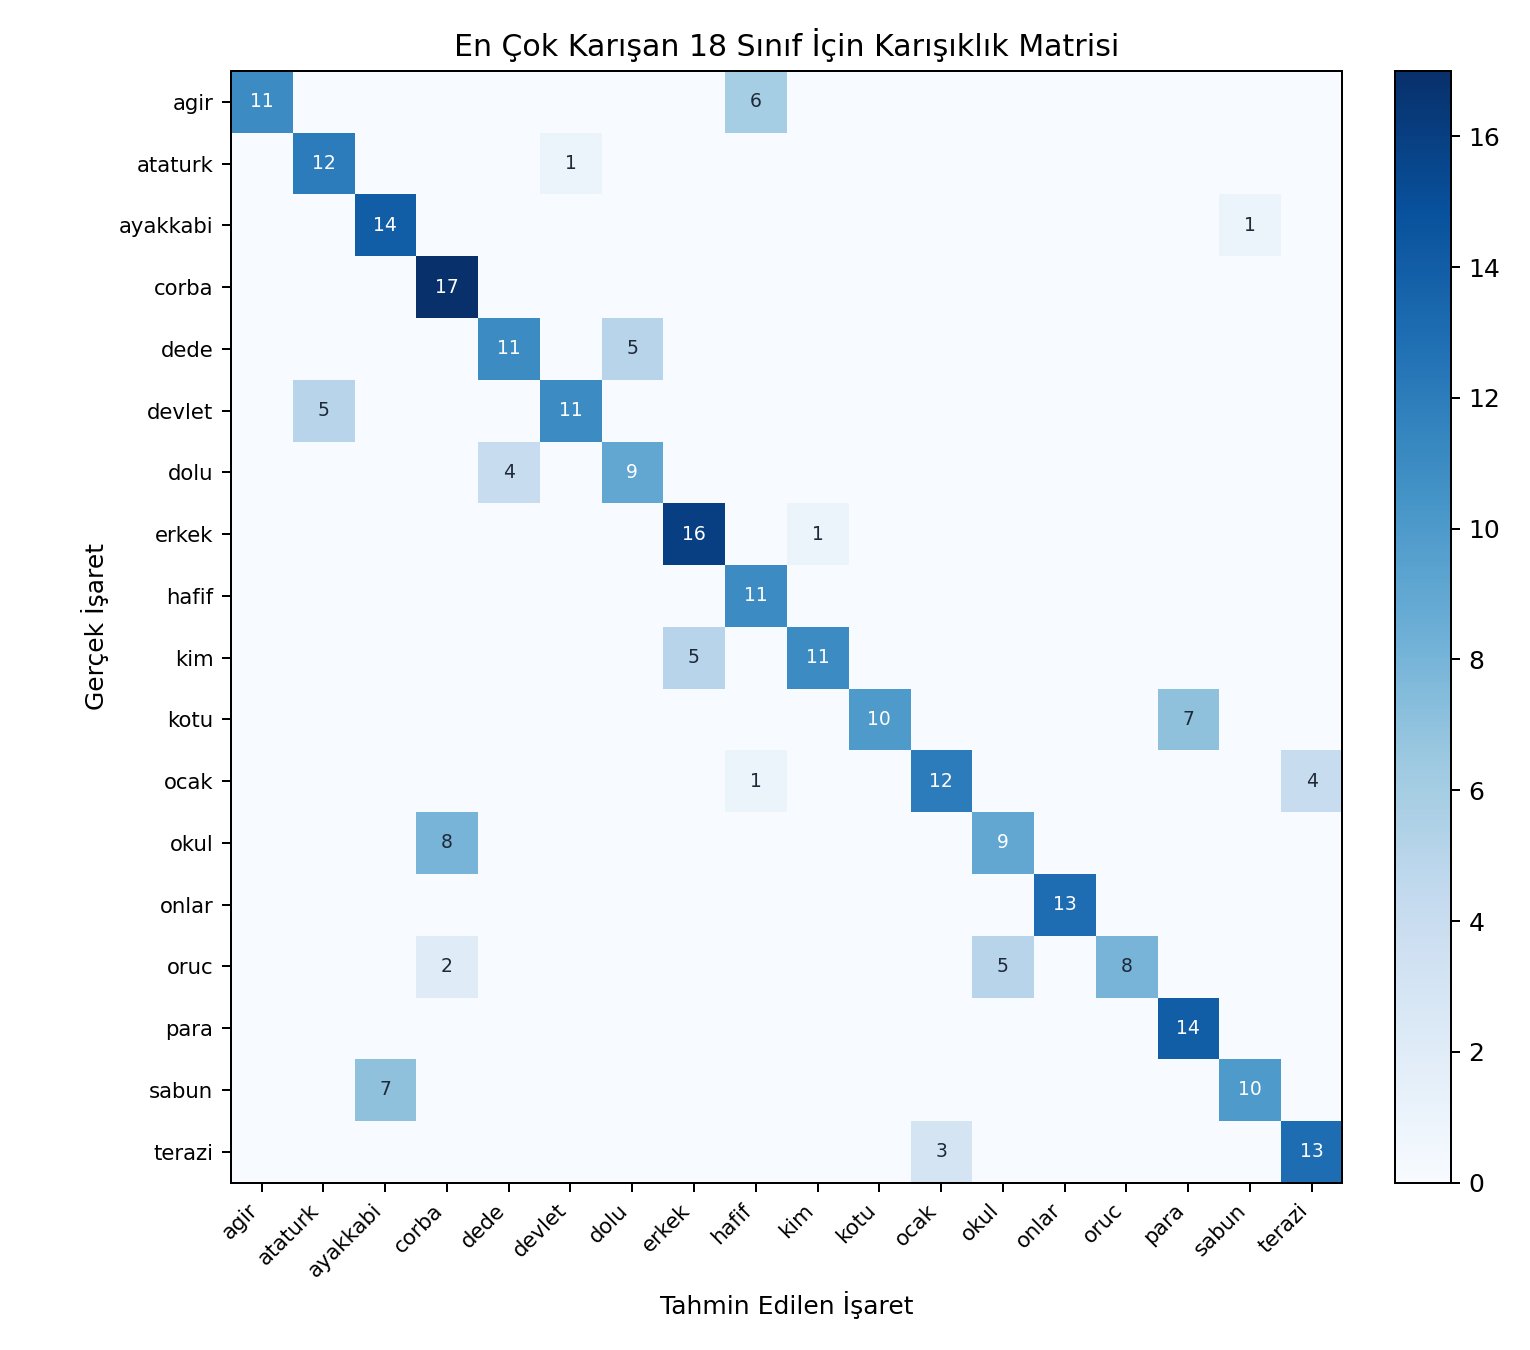
\includegraphics[width=0.8\textwidth]{grafik/karisiklik_matrisi.png}
\caption{Test kümesinde en çok karışan 18 sınıf için karışıklık matrisi (1B-CNN + Transformer, tohum 0)}
\label{fig:cm}
\end{figure}

\begin{table}[H]
\centering
\caption{Test kümesinde en sık karışan işaret çiftleri}
\label{tab:karisan}
\small
\begin{tabularx}{\textwidth}{@{}l l r X@{}}
\toprule
\textbf{Gerçek} & \textbf{Tahmin} & \textbf{Hata / Toplam} & \textbf{Olası neden} \\
\midrule
okul & çorba & 8 / 17 & İki elin göğüs önünde benzer kavisli hareketi \\
kötü & para & 7 / 17 & Parmak ucu sürtme hareketinin iki boyutta benzemesi \\
sabun & ayakkabı & 7 / 17 & İki elin birbirine sürtünme hareketi \\
ağır & hafif & 6 / 17 & Aynı el biçimi, yalnızca zıt yönde (aşağı/yukarı) hareket \\
oruç & okul & 5 / 16 & Ağız hizasında başlayan benzer el konumu \\
\bottomrule
\end{tabularx}
\end{table}

Hatalar rastgele dağılmamakta, el biçimi ve konumu aynı olup yalnızca ince parmak
teması ya da derinlik yönündeki hareketle ayrışan işaretlerde toplanmaktadır. En düşük
F1 skoruna sahip sınıflar \sol doktor\sag, \sol perşembe\sag, \sol dakika\sag{} ve
\sol yastık\sag{} olmuştur (F1 yüzde 48--54). Bu işaretlerin ayırt edici bilgisi
çoğunlukla parmakların yüze ya da birbirine değmesinde bulunmakta ve iki boyutlu
koordinatlarda zayıf kalmaktadır.

\subsection{Güven eşiği}

Model, sözlükte olmayan ya da yarım kalmış bir hareketi de 226 sınıftan birine atar. Bu
tür tahminleri ayıklamak için en yüksek softmax olasılığı üzerinde bir güven eşiği
uygulanmaktadır. Eşik, doğrulama kümesinde seçilip test kümesinde kontrol edilmiştir
(\texttt{calibrate\_threshold.py}). Uygulamadaki model için sonuçlar
Tablo~\ref{tab:esik} içindedir.

\begin{table}[H]
\centering
\caption{Güven eşiğine göre kabul oranı ve kabul edilenlerde doğruluk (1B-CNN + Transformer, test kümesi)}
\label{tab:esik}
\begin{tabular}{@{}rrr@{}}
\toprule
\textbf{Eşik} & \textbf{Kabul edilen (\%)} & \textbf{Kabul edilenlerde doğruluk (\%)} \\
\midrule
0 & 100,0 & 89,8 \\
0,5 & 88,7 & 95,0 \\
0,6 & 85,4 & 96,1 \\
0,7 & 80,2 & 97,0 \\
0,8 & 71,3 & 97,8 \\
\bottomrule
\end{tabular}
\end{table}

Uygulamada varsayılan eşik 0,6'dır ve kullanıcı ayarlardan değiştirebilir. Bu eşikte
test örneklerinin yüzde 85,4'ü kabul edilmekte ve bunlarda doğruluk yüzde 96,1'e
çıkmaktadır. Aynı eşikte BiGRU modeli örneklerin ancak yüzde 75'ini kabul
etmektedir. Elin hiç görünmediği yapay girdilerde modelin yine de bir kelime seçtiği
görüldüğünden, uygulamada kayıt boyunca el karelerin beşte birinden azında görünmüşse
kayıt modele verilmeden kullanıcı uyarılmaktadır.
